%% 和文論文用のテンプレート
%%%%%%%%%%%%%%%%%%%%%%%%%%%%%%%%%%%%%%%%%%%%%%%%%%%%%%%%%%%%%%%%%%%%%%%%%%%%
%% 1. 和文原稿
 \documentclass[originalpaper]{jsaiart}     % 原著論文 Original Paper
% \documentclass[blindreview]{jsaiart}      % 査読用
%
% \documentclass[shortpaper]{jsaiart}       % 速報論文 Short Paper
% \documentclass[exploratorypaper]{jsaiart} % 萌芽論文 Exploratory Research Paper
% \documentclass[Specialissue]{jsaiart}     % 特集 Special Issue
% \documentclass[specialissue]{jsaiart}     % 小特集 Special Issue
% \documentclass[interimreport]{jsaiart}    % 報告 An Interim Report
% \documentclass[surveypaper]{jsaiart}      % 解説 Survey Paper
% \documentclass[aimap]{jsaiart}            % AIマップ AI map
% \documentclass[specialpaper]{jsaiart}     % 特集論文 Special Paper
% \documentclass[invitedpaper]{jsaiart}     % 招待論文 Invited Paper
%

%% ページ番号の指定,掲載時に学会の方で決定します.
% \setcounter{page}{1}
% \setcounter{volpage}{1}


%%% amsmathパッケージの注意点 %%%%%%%%%%%%%%%%%%%%%%%%%%%%%%%%%%%%%%%
% \usepackpage{amsmath}
% 数式番号の参照は \ref ではなく,\eqref を用いること
% documentclass のオプションに fleqnを指定すること
% 例: \documentclass[technicalpaper,fleqn]{jsaiart}

\usepackage[dvipdfmx]{graphicx}
\usepackage{graphics}
\usepackage{fancybox}
\usepackage{comment}

\Vol{12}
\No{1}
%\jtitle{物体検出のためのニューラルネットワークのサーベイ}
\jtitle{物体検出に用いられるニューラルネットワークモデル}
% \jtitle[柱用和文タイトル]{和文タイトル}
\jsubtitle{最新モデルのサーベイと目的に応じたモデルの選択}
%\etitle{A Survey of Deep Neural Networks for Object Detection}
\etitle{Neural Network Models for Object Detection}
\esubtitle{A Survey of the Latest Models and Optimal Model Selections for Specific Tasks}

\manyauthor % 著者が3名以下の場合はこの行を消すこと

%%% 著者名の注意点 %%%%%%%%%%%%%%%%%%%%%%%%%%%%%%%%%%%%%%%%%%%%%%%%%%%
% 所属先が同じ著者が連続する場合,その中の先頭の著者のみ \affiliation
% を用い,残りの所属先には \sameaffiliation を使う
% ただし,所属先が同じでも連続していない場合は \affliation を使う
% 名前が長い場合は \name の代りに \longname を使う

\author{%
 \name{金子}{純也}{Junya Kaneko}
 \affiliation{Morning Project Samurai 株式会社}%
     {Morning Project Samurai Inc.}%
     {junya@mpsamurai.com, http://www.mpsamurai.com}
%\and
% \name{著者2姓}{名}{Auther2 Roman Name}
% \affiliation{日本語所属名2}%
%     {Affiliation2 in English}%
%     {user2@ai-gakkai.or.jp, http://www.ai-gakkai.or.jp/~user2/}
\and
 \name{山田}{貢己}{Miki Yamada}
 \sameaffiliation{m.yamada@mpsamurai.com}
%\and
% \longname{カタガナガキノ}{ナガイナガイナマエ}{VeryLong Roman Name}
% \sameaffiliation{user4@ai-gakkai.or.jp, http://www.ai-gakkai.or.jp/~user4/}
%\and
% \name{著者5姓}{名}{Auther5 Roman Name}
% \affiliation{日本語所属名1}%
%     {Affiliation1 in English}%
%     {user5@ai-gakkai.or.jp, http://www.ai-gakkai.or.jp/~user5/}
}

\begin{keyword}
%キーワードとして,小文字(固有名詞や略語を除く)の英単語を2〜5個指定
    survey, neural network, object detection, instance segmentation, deep learning
\end{keyword}

\begin{summary}
「ショートノート」は 200 ワード,それ以外は200〜500 ワード
以内の英文でsummaryを記す
(ここは,論文執筆後に書く.)
\end{summary}

\begin{document}
\maketitle

ここにチートシートを出力する.
\section{まえがき}
★作成中.
\section{物体検出(Object detection)}
%\begin{figure}[t]
%    \begin{center}
%        \includegraphics[width=8cm,clip]{fig/test_fig2.eps}
%    \end{center}
%    \caption{ 図の説明文 ... }
%\end{figure}    
\subsection{Two-stage検出器}
\subsubsection{Faster R-CNN}
\subsubsection{TFANet}
\subsubsection{Few-Shot Object Detection}
\subsection{One-stage検出器}
\subsubsection{YOLOv4}
\subsubsection{EfficientDet}
\section{インスタンスセグメンテーション(Instance segmentation)}
\subsection{Mask Scoring R-CNN (MS R-CNN)}
%\begin{figure*}[b] %これにすると独立したページに1段組で出力された.
\begin{figure}[b]
    \begin{center}
        \includegraphics[width=8cm,clip]{fig/archi_ms_rcnn.eps}
    \end{center}
    %\capwidth=90mm %
    \caption{ Mask Scoring R-CNN の構造.}
    %\end{figure*}
    \label{fig:archi_ms_rcnn}
\end{figure}
マスク品質(インスタンスマスクと正解マスクとのIoUとして定量化されるもの)を分類スコアと明示的に関連付けたモデルである\cite{HHGHW19}.MS R-CNN は,予測マスクの品質を学習するためのブロック(MaskIoU Head)を,Mask R-CNN\cite{HGDG17} に導入したモデルになっている(\ref{fig:archi_ms_rcnn}).MaskIoU Headはインスタンスの特徴量と対応する予測マスクを一緒に取り込み,それを元にMask IoU を回帰推定する.そして,推論時に予測MaskIoUを分類スコアに掛け算して補正する.
\subsubsection{MS R-CNN の学習}
学習サンプルとして RPN proposals を使う.
proposal box と正解box との IoU が 0.5 以上の学習サンプルが必要となる.これは Mask R-CNN の Mask head の学習サンプルの場合と同じである.
各学習サンプルに対する回帰目標を生成するために,まず目標クラスの予測マスクを取得し,予測マスクを閾値=0.5で2値化する.そして,2値化マスクと正解との MaskIoU を使う.
MaskIoUを回帰するのには L2 損失を使い,損失重みは1にする.
ネットワーク全体は end-to-end で学習する.
\subsubsection{MS R-CNN の推論処理}
MaskIoU Head は分類スコア(R-CNN head の出力)の調整に使う.推論の手順は次のようになる:
\begin{enumerate}
    \item R-CNN head が $N$個のbounding boxを出力する.
    \item $N$個のbounding boxのうち,SoftNMS\cite{BSCD17}で上位$k$個のボックスを選択する.
    \item 上位$k$個のボックスを Mask Head に入力し,$k$個のマルチクラスマスクを生成する(ここまでは標準的 Mask R-CNN の手順).
    \item これら$k$個のマスクを目標として MaskIoU Head に入力し,予測 MaskIoU を出力する.
    \item 予測 MaskIoU を,分類スコアに掛け算し,上位$k$個の修正された分類スコアを得る.
\end{enumerate}

\subsection{YOLACT++}
\section{パノプティックセグメンテーション(Panoptic(?) segmentation)}
\section{むすび}

\begin{acknowledgment}
謝辞について
\end{acknowledgment}

%\bibliography{btxsample}
\bibliography{mps}
\bibliographystyle{jsai}

\appendix

\section{付録のタイトル1}
付録の本文1
%\section{付録のタイトル2}
%付録の本文2

% 著者の姓と名の間は半角スペースで区切る
% 略歴は200字以内
\begin{biography}
    %\profile*{m}{著者姓 名}{前掲\kern-.5zw (Vol.X,No.Y,p.Z)\kern-.5zw 参照.}
\profile{m}{金子 純也}{著者1の略歴}
\profile{m}{山田 貢己}{1989年東京大学大学院物理学専攻修了.理学博士.同年株式会社東芝入社.ニューラルネットワークの研究開発,セキュリティ技術,画像認識技術,テレビの高画質化技術,車載画像認識プロセッサ等の開発業務に従事.2020年ジャパニアス株式会社に入社.現在,Morning Project Samurai 株式会社においてAI開発業務に従事.}
\end{biography}

\end{document}
